\input{Formato/formatoMEI}


\instituto{Universidad Tecnológica Nacional\\Facultad Regional Córdoba}
\carrera{Ingeniería Electrónica}
\title{Análisis de señales y Mediciones básicas con Osciloscopios}
\subtitledoc{Trabajo Práctico de Laboratorio Nº 2}
\professor{
   JTP Ing. Luis Alberto Guanuco, \par
   Ing. Carlos Centeno, \par
   Ing. Martín Salamero.
}
\catedra{Medidas Electrónicas I}
\curso{4R1}
\author{
    Robertson, Máximo. \par 
    Musso, Lucas.  \par 
    Arenas, Nicolás. \par 
    Palacios, Alexandro. \par 
}
\legajo{
    89712 \par 
    91934 \par 
    86607 \par 
    91454 \par
}
\footerauthor{
Robertson, Musso, Arenas, Palacios.
}
\footerlegajo{  
    89712, 91934, 86607, 91454.
}


\begin{document}
\maketitle

\tableofcontents
\newpage


\section{Introducción}
%En este segundo trabajo práctico de laboratorio de la materia Medidas Electrónicas I, se analizarán y medirán señales en el dominio del tiempo con osciloscopios tanto analógicos como digitales. En esta oportunidad, se realizarán múltiples experimentos donde se verán de manera práctica los conceptos aprendidos en clase, con el objetivo de adquirir experiencia en el uso de osciloscopios para efectuar el análisis y la medición de algunos parámetros en distintos tipos de formas de ondas.
\section{Introducción}
\subsection{Roles de los Integrantes}

La división de las tareas dentro de nuestro grupo en este trabajo será la siguiente: 

\begin{table}[h!]
    \centering
    \begin{tabular}{|c|c|}
    \hline
        Alumno & Rol \\
    \hline
        Musso, Lucas & Coordinador \\ 
        Arenas, Nicolás & Operador 1 \\
        Palacios, Alexandro & Operador 2 \\
        Robertson, Máximo & Documentación \\
    \hline
        \end{tabular}
        \def\tablename{Tabla} 
        \caption{Tabla de asignación de roles para cada integrante}
        \label{tab:roles}
\end{table}

La fecha de entrega estipulada en el cronograma entregado a los docentes para este trabajo práctico es del \textbf{\textit{25 de abril del 2024}}.

Y la fecha en que el equipo rendirá el coloquio oral será también el día \textbf{\textit{25 de abril del 2024}}.



\subsection{Grilla de Evaluación}

\begin{table}[H]
    \centering
    \scalebox{0.895}{
    \begin{tabular}{|c|p{6.5cm}|c|c|c|c|c|}
    \hline
        \multirow{2}{*}{ID} & \multirow{2}{*}{Criterio de Evaluación} & \multicolumn{4}{c|}{\%Obt.} & \multirow{2}{*}{\%max} \\ 
        \cline{3-6}
        ~ & ~ & ECG & EO1 & EO2 & ED & ~ \\ \hline
        CEval 1 & Identifica los datos necesarios para determinar especificaciones de los instrumentos disponibles & ~ & ~ & ~ & ~ & 5\% \\ \hline
        CEval 8 & Identifica los elementos necesarios para realizar el trabajo requerido & ~ & ~ & ~ & ~ & 5\% \\ \hline
        CEval 10 & Adquiere los conocimientos necesarios para la correcta implementación del procedimiento de medición & ~ & ~ & ~ & ~ & 5\% \\ \hline
        CEval 5 & Trabaja en forma grupal para completar todas las tareas establecidas en el procedimiento indicado para la realización del trabajo practico & ~ & ~ & ~ & ~ & 10\% \\ \hline
        CEval 11 & Realiza los cálculos necesarios para determinar de forma empírica los parámetros de los amplificadores en cada una de las configuraciones planteadas & ~ & ~ & ~ & ~ & 5\% \\ \hline
        CEval 13 & Realiza los cálculos requeridos para determinar los parámetros del amplificador en las configuraciones planteadas de forma analítica & ~ & ~ & ~ & ~ & 5\% \\ \hline
        CEval 14 & Realiza las mediciones para determinar los parámetros del amplificador en las configuraciones planteadas de forma empírica & ~ & ~ & ~ & ~ & 10\% \\ \hline
        CEval 23 & Hace búsqueda y selección de información  relevante para validar las mediciones realizadas & ~ & ~ & ~ & ~ & 5\% \\ \hline
        CEval 4 & Documenta con información precisa el resultado de las mediciones. & ~ & ~ & ~ & ~ & 10\% \\ \hline
        CEval 12 & Evalúa los resultados de las mediciones para determinar la validez de las mismas & ~ & ~ & ~ & ~ & 10\% \\ \hline
        CEval 3 & Realiza el informe técnico con información precisa para dar a conocer los resultados de las mediciones & ~ & ~ & ~ & ~ & 10\% \\ \hline
        CEval 7 & Expone de forma grupal inconvenientes, experiencia generada y conclusiones acerca del trabajo realizado & ~ & ~ & ~ & ~ & 10\% \\ \hline
        CEval 32 & Expone de forma individual inconvenientes, experiencia generada y conclusiones acerca del trabajo realizado & ~ & ~ & ~ & ~ & 10\% \\ \hline
        ~ & TOTAL & ~ & ~ & ~ & ~ & 100\% \\ \hline
    \end{tabular}}
    \def\tablename{Tabla} 
    \caption{Grilla de Evaluación}
\end{table}
\vspace{2cm}
\section{Materiales e Instrumentos}
Los instrumentos y materiales utilizados a lo largo de todo este trabajo práctico, son los siguientes:

\begin{itemize}
    \item Osciloscopios Analógicos: marca PINTEK, modelo PS-200; marca LEADER, modelo 8041.
    \item Osciloscopio Digital: marca RIGOL, modelo DS1052E.
    \item 2 Puntas de Osciloscopio Hantek de 100 Mhz.
    \item Generador de funciones: marca GW INSTEK, modelo GFG 3015.
    \item Fuente de tensión variable del laboratorio central de la UTN-FRC.
    \item Kit del TP2 de Medidas Electrónicas (disponible en el laboratorio central de electrónica de la UTN-FRC). Contiene una fuente con salida regulada y no regulada de aprox 12V; un circutio generador de una onda de aprox. 400 Hz; un marcador de teléfono antiguo (disco) con un circuito incorporado para poder ver las señales; y una placa auxiliar para generar un tren de pulsos diferencial.
    
\end{itemize}

\newpage
\section{Marco teórico}
\subsection{Potencia Eléctrica}
La potencia eléctrica es una medida de la cantidad de energía que se consume, produce o transfiere en un circuito eléctrico en un período de tiempo determinado. Es un concepto fundamental en el estudio y diseño de sistemas eléctricos y electrónicos. 
Cuando se trata de corriente continua (CC) la potencia eléctrica desarrollada en un cierto instante por un dispositivo de dos terminales, es el producto de la diferencia de potencial entre dichos terminales y la intensidad de corriente que pasa a través del dispositivo. Por esta razón la potencia es proporcional a la corriente y a la tensión

\begin{equation}
    P= V \cdot I 
\end{equation}

En cambio, cuando se trata de corriente alterna (AC) sinusoidal, el promedio de potencia eléctrica desarrollada por un dispositivo de dos terminales es una función de los valores eficaces o valores cuadráticos medios, de la diferencia de potencial entre los terminales y de la intensidad de corriente que pasa a través del dispositivo. 


Existen 3 tipos de potencias presentes en un circuito de CA, la potencia activa, la potencia reactiva y la potencia aparente. La relación entre estas se puede observar a través del llamado triangulo de potencias. 

\begin{figure}[h]
    \centering
    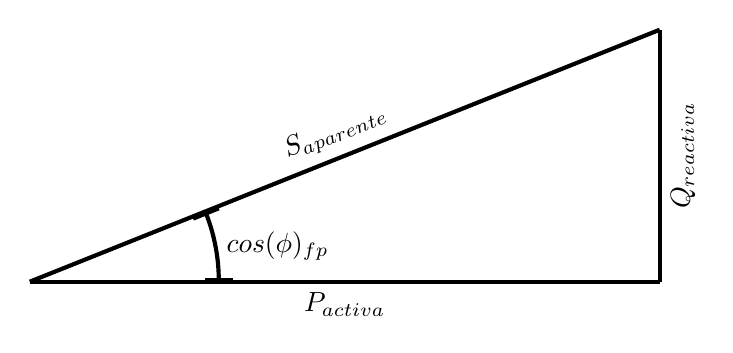
\begin{tikzpicture}[scale=0.8]
    \draw[line width = 1.5pt, black] (0,0)--(10,0) node[midway, below]{$P_{activa}$};
    \draw[line width=1.5pt, black](10,0)--(10,4) node[midway,below,sloped]{$Q_{reactiva}$};
    \draw[line width=1.5pt,black](10,4)--(0,0) node[sloped,midway,above]{$S_{aparente}$};
    \draw[line width=1.5pt,black,|-|](3,0) arc (0:21.8:3) node[midway,right]{$cos(\phi)_{fp}$};
\end{tikzpicture}
    \caption{Triángulo de potencias}
    \label{fig:triang_pot}
\end{figure}
\subsubsection{Potencia activa}
Es la potencia capaz de transformar la energía eléctrica en trabajo. Los diferentes dispositivos eléctricos existentes convierten la energía eléctrica en otras formas de energía tales como: mecánica, lumínica, térmica, química, etc. Esta potencia es, por lo tanto, la realmente consumida por los circuitos y, en consecuencia, cuando se habla de demanda eléctrica, es esta potencia la que se utiliza para determinar dicha demanda. 
Se designa con la letra (\textbf{P}) y se mide en vatios —watt— (W) o kilovatios —kilowatt— (kW).
\begin{equation}
    P=  V\cdot I\cdot\cos \phi
\end{equation}

\subsubsection{Potencia reactiva}
La potencia reactiva es la potencia que fluye entre el equipo eléctrico y la fuente de alimentación debido a la capacitancia o inductancia del equipo. No realiza trabajo útil en el circuito, sino que se intercambia entre la fuente de energía y los dispositivos inductivos o capacitivos. Su efecto principal es el almacenamiento y la liberación de energía magnética.
Se representa con la letra (\textbf{Q}) y Se mide en voltamperios reactivos (VAR).

\begin{equation}
    Q = V\cdot I\cdot\sen \phi
    \label{eq:visenphi}
\end{equation}

\subsubsection{Potencia aparente}
La potencia aparente (\textbf{S)} es la suma vectorial de la potencia activa y la potencia reactiva. Se mide en voltamperios (VA). Representa la magnitud total de la potencia que fluye en un circuito, incluyendo tanto la potencia activa como la reactiva. Es la potencia que se observaría si solo se midieran los voltajes y corrientes en el circuito y si no existiera un desfasaje entre ellos. 
\begin{equation}
    S= V \cdot I
\end{equation}

\subsection{Factor de potencia}
Como ya se explicó, la energía presente en un sistema
de corriente alterna en régimen permanente está compuesta por una parte
que realiza un trabajo y por otra parte que se almacena
en los elementos reactivos y se intercambia con la fuente. La relación que existe entre la energía aprovechada (la que es capaz de realizar un trabajo) y la energía total disponible se conoce como \textit{factor de potencia} ($\mathrm{fp}$). Estas energías se relacionan con la siguiente expresión:

\begin{equation}
    \mathrm{fp} = \frac{P}{S} = \cos(\phi)
\end{equation}

Por su definición, el factor de potencia es el rendimiento del sistema, y
como tal, es un número adimensional comprendido entre 0 y 1. Un factor de potencia cercano a 1 indica que la mayor parte de la energía es utilizada para realizar trabajo.

\label{sec:fp}
\subsubsection{Corrección del factor de potencia}
La energía transportada que no se consume produce pérdidas, sobrecarga los transformadores y por lo tanto disminuye la eficiencia del sistema eléctrico en general. Es por esta razón que es deseable corregir el valor de $\mathrm{fp}$ y llevarlo lo más cercano a 1 para mejorar el rendimiento del sistema. La corrección del factor de potencia se logra conectando al sistema cargas reactivas (generalmente en paralelo para no modificar la tensión aplicada) de naturaleza contraria a la que el sistema tiene. Normalmente se trata de sistemas resistivo-inductivos los que se necesita compensar, por lo que se utilizarán cargas capacitivas para la corrección.
Por lo tanto, dado un $\mathrm{fp} = \cos \phi$ y una pulsación de red $\omega$, el valor de capacitancia paralela necesario para llevar el factor de potencia a 1 se calcula con la expresión:

\begin{equation}
    C = \frac{P\cdot \tan\phi}{V^2\cdot \omega}
    \label{eq:corrFp}
\end{equation}


\subsection{Voltímetros de CA}
\label{sec:VoltCA}

Los voltímetros de corriente alterna, son instrumentos de medición que nos entregan el valor numérico de la tensión eficaz de la señal medida.

La gran mayoría de los voltímetros para CA usados en electrónica, vienen preparados para medir tensión únicamente sobre ondas senoidales o cosenoidales. Estos utilizan conversores (o detectores) de respuesta al valor medio y estan calibrados para indicar el valor eficaz, mediante la aplicación de un factor que relaciona los valores “medio de módulo” y “eficaz”, pero como se mencionó solo para ondas sinusoidales. 

Si con esta clase de instrumento se intenta medir tensiones provenientes de fuentes que entregan otros tipos de formas de onda (como pueden ser; ondas cuadradas, triangulares, trenes de pulsos, senoidales controladas por SCR o Triacs, etc.), aparecerá un error porque el factor de calibración que debería aplicarse es distinto para cada caso. 

Se pueden eliminar estos errores si se conocen con exactitud el tipo de forma de onda de que se trata, ya que en cada situación es posible aplicar ciertas cotas de corrección que pueden deducirse en forma analítica o que pueden determinarse directamente mediante mediciones.

Sin embargo, existe otra clase de voltímetro de CA, llamado \textbf{True RMS}, el cual identifica la forma de onda de la señal medida, y en base a esta, aplica el factor de corrección correspondiente. De este modo, este tipo de instrumentos permite medir directamente la tensión eficaz, sin necesidad de cálculos adicionales.

De todas maneras, se debe tener en cuenta que cuando la señal medida no es sinusoidal, la exactitud de la precisión se ve afectada y el nuevo porcentaje de error estará directamente afectado por el factor de cresta de la onda.

\subsection{Factor de Cresta}

Se conoce como factor de cresta al cociente entre el valor máximo y el valor eficaz de la señal.
\begin{equation}
    F_c = \cfrac{V_p}{V_ef}
\end{equation}

A continuación se muestran las fórmulas para algunos factores de cresta, de las señales más comunes (figura \ref{fig:facCrest}). $V$ representa el valor pico de la señal en cuestión.

\begin{figure}[H]
    \centering
    \includegraphics[width=0.4\linewidth]{Imagenes/FacCrest.jpg}
    \caption{Factores de Cresta de las señales más comunes}
    \label{fig:facCrest}
\end{figure}




%El propósito de este trabajo es justamente obtener en forma práctica dichas cotas para un determinado instrumento, comparando su respuesta con la de uno que usa detector de respuesta al valor eficaz verdadero, ya que, en principio, este tipo de voltímetro es capaz de medir cualquier forma de onda. 




\newpage
\section{Desarrollo}

\vspace{0.5cm}
\subsection{Experimento 1: Experiencias con osciloscopio analógico}

\vspace{0.5cm}
\subsubsection{Aprendiendo a calibrar (compensar) la punta atenuadora}

Con este primer experimento, se pretende demostrar la importancia de la calibración de la punta de medición mediante una comparativa entre los tres tipos posibles de compensación (figura \ref{calib}).

%figura de los tres tipos de compensación

\begin{figure}[H]
    \centering
    \includegraphics[width=\textwidth]{Imagenes/calib.png}
    \caption{Tipos de compensación con la punta de osciloscopio}
    \label{calib}
\end{figure}

Para comenzar, se puso el seleccionador de la punta en la opción de "X10", esto con el fin de aumentar considerablemente su resistencia de entrada al osciloscopio y disminuir su capacidad paralela de entrada, reduciendo al mínimo la influencia de la conexión del instrumento sobre el circuito a medir.

Se procedió a ajustar el capacitor de compensación en el conector de la punta hasta lograr cada una de las formas de onda. %indicas en la figura \ref{}. 

Los parámetros del osciloscopio fueron ajustados de la siguiente manera (tabla \ref{tab:cont1}):

\begin{table}[H]
    \centering
    \scalebox{1}{
    \begin{tabular}{|c|c|c|c|c|}
    \hline
         V/div (C. Y1) & t/div (B. tiempo) & Aten. Y1 & Acoplamiento & Disparo \\
    \hline
        50 $mV$ & 0.2 $ms$ & x10 & CC & CH1\\
    \hline
        \end{tabular}}
        \def\tablename{Tabla} 
        \caption{Cuadro de Controles}
        \label{tab:cont1}
\end{table}

Las señales obtenidas, se presentan a continuación (figura \ref{compen})

%foto triple de las señales del osc

\begin{figure}[H]
    \begin{center}
        \begin{subfigure}[t]{0.5\textwidth}
        \centering  
        \includegraphics[width=0.75\textwidth]{Imagenes/SigA.jpeg}
        \caption{Compensación A}
        \label{fig:sigA}
    \end{subfigure}
    \hfill
    \begin{subfigure}[t]{0.49\textwidth}
        \centering
        \includegraphics[width=0.77\textwidth]{Imagenes/SigB.jpeg}
        \caption{Compensación B}
        \label{fig:sigB}
    \end{subfigure}
    \begin{subfigure}[t]{0.5\textwidth}
        \centering
        \includegraphics[width=0.75\textwidth]{Imagenes/SigC.jpeg}
        \caption{Compensación C (punta calibrada)}
        \label{fig:sigC}
    \end{subfigure}
    \caption{Señal de prueba con los tres tipos de calibración}
    \label{compen}
    \end{center}
\end{figure}

Una vez obtenida la señal de la figura \ref{fig:sigA}, se procedió a conectar un generador de funciones configurado para generar una onda sinusoidal y se realizó un barrido manual de frecuencia, desde 100 Hz hasta 1 MHz. Se tomó nota de la amplitud observada en cada instancia de frecuencia y se confeccionó una tabla con los datos. 

Debido a que había que realizar el mismo procedimiento para los tres tipos de compensación, se decidió ubicar todos los datos en una misma tabla para mayor legibilidad y para poder comparar los efectos en cada caso con mayor facilidad.

Para el barrido, se empleó una señal sinusoidal de 1 Vpp (que será visto como 100 mVpp por la punta al estar en X10), y la frecuencia fue variada según lo que se observa en la tabla. Para esta parte también se cambió la escala del osciloscopio a 20 mV/div para poder apreciar con más detalle los cambios de amplitud.

%Tabla de barrido de frecs

\begin{table}[H]
    \centering
    \scalebox{1}{
    \begin{tabular}{|c||c||c|c|c|}
    
    \hline
         \multirow{2}{*}{$f$ [Hz]} & \multirow{2}{*}{t/div [$\mu$s]} & \multicolumn{3}{c|}{Amplitud $[mVpp]$} \\
    \cline{3-5}
          &  & Comp. a) & Comp. b) & Comp. c) \\
    \hline
        100 & 2000 & 100 & 100 & 100 \\
        1k & 200 & 112 & 90 & 100 \\
        10k & 20 & 120 & 84 & 100 \\
        100k & 2 & 120 & 82 & 100 \\
        250k & 1 & 120 & 81 & 100 \\
        1M & 0.2 & 120 & 80 & 100 \\ 
    \hline
        \end{tabular}}
        \def\tablename{Tabla} 
        \caption{Barrido en frecuencia para las distintas compensaciones}
        \label{tab:BarrFrec}
\end{table}

Se puede ver, en base a los valores obtenidos, que en el único modo de compensación en el que las mediciones no variaron al cambiar la frecuencia, fue con el modo \textit{c)} (figura \ref{fig:sigC}). En los otros dos modos, la señal de entrada al osciloscopio se vio afectada por la variación de frecuencia, aumentando el valor de la señal medida en el modo \textit{a)} y disminuyéndolo en \textit{b)}.

En la hoja de enunciados se solicitaba completar una serie de frases con cada modo y estas quedan de la siguiente manera:

\begin{enumerate}
    \item El oscilograma \textbf{\textit{b)}} corresponde a “caída de respuesta en frecuencias elevadas”.
    \item El oscilograma \textit{\textbf{a)}} corresponde a “exceso de respuesta en frecuencias elevadas”.
    \item El oscilograma \textbf{\textit{c)}} corresponde a “respuesta plana”.
\end{enumerate}





\vspace{0.5cm}
\subsubsection{Acoplamiento \textit{CC/CA} de la entrada vertical (eje Y)}

En este ensayo se pretende visualizar el efecto de la capacitancia de entrada del osciloscopio cuando este se encuentra en acoplamiento de \textit{CA}.

En este modo, la entrada del eje Y del osciloscopio tiene conectado internamente, un capacitor en serie que bloquea la componente de \textit{CC} y este en ciertos casos (sobre todo a bajas frecuencias) puede provocar deformaciones en la forma de la onda. 

Para este experimento, se empleará nuevamente un generador de onda, pero esta vez se inyectara una onda cuadrada, con frecuencia de 50 Hz y amplitud de 20 $V_{pp}$ (máxima del generador). 

Inicialmente las configuraciones del osciloscopio y la punta serán las siguientes:

\begin{table}[H]
    \centering
    \scalebox{1}{
    \begin{tabular}{|c|c|c|c|}
    \hline
         V/div (C. Y1) & t/div (B. tiempo) & Aten. Y1 & Disparo \\
    \hline
        5 $V$ & 2 $ms$ & x1 & LINE\\
    \hline
        \end{tabular}}
        \def\tablename{Tabla} 
        \caption{Cuadro de Controles}
        \label{tab:cont2}
\end{table}

Se establece como fuente de disparo la opción \textit{LINE}, ya que la tensión de línea tiene una frecuencia de 50 Hz, coincidente con la señal producida por el generador. Esto debería garantizar la estabilidad de la imagen a la hora de verla en el osciloscopio.

Primeramente se selecciona la opción de acoplamiento en \textit{CC} y como era de esperarse, se muestra en pantalla una señal cuadrada sin distorsión. (figura \ref{dcx1}).

Luego se pasa a la opción de acoplamiento de \textit{CA}, la cual deforma la onda y donde antes se veían lineas horizontales (picos y valles), ahora se ven líneas con pendientes (figura \ref{acx1}).

%Imagen de las dos ondas (subfigure)

\begin{figure}[H]
    \begin{center}
        \begin{subfigure}[b]{0.5\textwidth}
        \centering  
            \includegraphics[width=0.75\textwidth]{Imagenes/DCx1.jpeg}
        \caption{Acoplamiento en CC}
        \label{dcx1}
    \end{subfigure}
    \hfill
    \begin{subfigure}[b]{0.49\textwidth}
        \centering
            \includegraphics[width=0.77\textwidth]{Imagenes/ACx1.jpeg}
        \caption{Acoplamiento en CA}
        \label{acx1}
    \end{subfigure}
    \caption{Señal de prueba con distintos acoplamientos y punta en atenuación x1}
    \end{center}
\end{figure}

En las imágenes se ven algunos pulsos más luminosos que otros debido a que al ser una frecuencia tan baja (50 Hz), la cámara que tiene una frecuencia de muestreo de 60 Hz, sacaba las fotos tan "rápido" que la imagen no llegaba a completarse.  

Para tratar de mitigar el efecto de este capacitor de entrada, se nos propuso cambiar la atenuación de la punta a \textit{x10}, manteniendo la onda del generador. También se actualizaron las configuraciones del osciloscopio para ver correctamente la señal (tabla \ref{tab:cont2b}).

\begin{table}[H]
    \centering
    \scalebox{1}{
    \begin{tabular}{|c|c|c|c|}
    \hline
         V/div (C. Y1) & t/div (B. tiempo) & Aten. Y1 & Disparo \\
    \hline
        500 $mV$ & 2 $ms$ & x10 & LINE\\
    \hline
        \end{tabular}}
        \def\tablename{Tabla} 
        \caption{Cuadro de Controles}
        \label{tab:cont2b}
\end{table}

Nuevamente, conectamos el generador y pusimos el acople en \textit{CC} y en \textit{CA}. Los resultados se pueden ver en la figura \ref{fig:x10}.

%Imagen de las ondas con la punta en x10 (subfigure)

\begin{figure}[H]
    \label{fig:x10}
    \begin{center}
        \begin{subfigure}[b]{0.5\textwidth}
        \centering  
            \includegraphics[width=0.75\textwidth]{Imagenes/DCx10.jpeg}
        \caption{Acoplamiento en CC}
        \label{dcx10}
    \end{subfigure}
    \hfill
    \begin{subfigure}[b]{0.49\textwidth}
        \centering
            \includegraphics[width=0.77\textwidth]{Imagenes/ACx10.jpeg}
        \caption{Acoplamiento en CA}
        \label{acx10}
    \end{subfigure}
    \caption{Señal de prueba con distintos acoplamientos y punta en atenuación x10}
    \end{center}
\end{figure}

Con el acople de \textit{CC} la señal se muestra prácticamente igual que en el caso anterior también con \textit{CC}. Pero en la figura \ref{acx10}, correspondiente al acople en \textit{CA}, se puede ver que aunque siguen existiendo, las pendientes de las lineas han disminuido considerablemente (llegando al punto de casi no notarse). 
%Esto se debe a la capacitancia



\vspace{0.5cm}
\subsubsection{Midiendo Componentes de $V_{CA}$ con un osciloscopio – Disparo por “LINEA”}

Este ensayo se realiza con el objetivo de apreciar el efecto de utilizar el disparo por "LINEA" de la opción de la fuente de TRIGGER del osciloscopio, con el objetivo de visualizar de manera estable una señal o ruidos acoplados provenientes de la red eléctrica de linea.

Para ello se utilizó una fuente de baja tensión que contaba con dos salidas, una de ellas estaba regulada y marcaba 12V y la otra estaba sin regular. Luego se conectó en la salida regulada una resistencia de $39 \Omega$ ($5 W$) que será utilizada como carga. 

Si bajo estas condiciones se midiera la tensión de salida sin regular, se podrá apreciar que la señal tendrá acoplado el efecto de ripple proveniente de la etapa de filtrado previa. Es posible aproximar el valor de tensión continua de la señal si se configura el osciloscopio correctamente. El primer paso es llevar el selector de acoplamiento de entrada del canal a la
posición "GND" (entrada a masa) y ajustar la línea de base en una posición de referencia cómoda para tomar la medición. Luego se retorna el selector de acoplamiento a CC, y se configura el oscilospio para visualizar correctamente la señal.

\begin{table}[H]
    \centering
    \scalebox{1}{
    \begin{tabular}{|c|c|c|c|}
    \hline
         V/div (C. Y1) & t/div (B. tiempo) & Aten. Y1 & Disparo \\
    \hline
        0.5 $V$ & 2 $ms$ & x10 & INTERNO\\
    \hline
        \end{tabular}}
        \def\tablename{Tabla} 
        \caption{Cuadro de Controles}
        \label{tab:cont3}
\end{table}

Se conecta la punta a la salida no regulada como se observa en las figuras \ref{fig::MedSalNoRegulada1} y \ref{fig::MedSalNoRegulada2}, y se procede a calcular el voltaje multiplicando la cantidad de divisiones que se desplaza la línea sobre la pantalla por el valor de escala vertical utilizado, teniendo en cuenta que la punta se encuentra atenuada X10. El resultado de la medición fue:

$$V_{CC} = 24V$$

\begin{figure}[H]
        \begin{subfigure}[b]{0.5\textwidth}
        \centering  
        \includegraphics[width=0.85\textwidth]{Imagenes/Ensayo 3-1.jpeg}
        \caption{Medición Salida no regulada (vista 1)}
        \label{fig::MedSalNoRegulada1}
    \end{subfigure}
    \hfill
    \begin{subfigure}[b]{0.49\textwidth}
        \centering
        \includegraphics[width=0.7\textwidth]{Imagenes/Ensayo 3-2.jpeg}
        \caption{Medición Salida no regulada (vista 2)}
        \label{fig::MedSalNoRegulada2}
    \end{subfigure}
    \caption{Circuito de fuente regulada y no regulada, con punta en la salida no regulada}
\end{figure}


El siguiente paso del ensayo, es intentar visualizar el ripple superpuesto a la tensión de $V_{CC}$ que se está midiendo. Para ello habrá que llevar el acoplamiento a CA y se elige una configuración de escala vertical adecuada:

\begin{table}[H]
    \centering
    \scalebox{1}{
    \begin{tabular}{|c|c|c|c|}
    \hline
         V/div (C. Y1) & t/div (B. tiempo) & Aten. Y1 & Disparo \\
    \hline
        50 $mV$ & 2 $ms$ & x10 & INTERNO\\
    \hline
        \end{tabular}}
        \def\tablename{Tabla} 
        \caption{Cuadro de Controles}
        \label{tab:cont3b}
\end{table}

Se observa que el disparo está configurado en "INTERNO", lo cual produjo dificultades a la hora de ajustar el disparo. La forma correcta de realizar estas mediciones es utilizando el disparo por "LINEA", ya que la frecuencia del ruido debe ser múltiplo de la frecuencia de la tensión de línea (50 Hz). Utilizando esta nueva configuración:

\begin{table}[H]
    \centering
    \scalebox{1}{
    \begin{tabular}{|c|c|c|c|}
    \hline
         V/div (C. Y1) & t/div (B. tiempo) & Aten. Y1 & Disparo \\
    \hline
        50 $mV$ & 2 $ms$ & x10 & LINEA\\
    \hline
        \end{tabular}}
        \def\tablename{Tabla} 
        \caption{Cuadro de Controles}
        \label{tab:cont3c}
\end{table}

El valor pico a pico del ripple teniendo en cuenta la atenuación es de:

$$V_{pp_{ripple}} = 2.3V$$

En la hoja de enunciados se solicitaba completar una serie de frases sobre las características del ripple y estas quedan de la siguiente manera:

\begin{enumerate}
    \item La frecuencia del ripple superpuesto es \textit{\textbf{100}} Hz. 
    
    Esto es debido a que luego de la rectificación en el puente de diodos, queda una señal pulsante del doble de la frecuencia de la señal de entrada, en este caso la frecuencia de línea (50 Hz).
    \item El porcentaje de ripple respecto del valor de $V_{CC}$ es del \textbf{\textit{9.583}} \%.
\end{enumerate}

\begin{figure}[H]
    \centering
    \includegraphics[width=0.6\textwidth]{Imagenes/Ensayo 3-3.jpeg}
    \caption{Medición del Ripple}
    \label{fig::MedicionRipple}
\end{figure}

\vspace{0.5cm}
\subsubsection{Usando el disparo (trigger) interno de un osciloscopio} 

Esta sección estará dedicada a comprender como funcionan algunos controles más específicos del \textit{Trigger} o disparo. En este caso, se utilizará como fuente de disparo, el trigger interno, en este caso se utilizo la señal de disparo del canal 1 (CH1).

Para comenzar, se ajustará el generador de funciones para que proporcione una onda sinusoidal, con frecuencia de 500 Hz y una amplitud de 2,5 V (Voltaje pico). 

Los parámetros para la punta y el osciloscopio serán los siguientes (tabla \ref{tab:cont4}):

\begin{table}[H]
    \centering
    \scalebox{1}{
    \begin{tabular}{|c|c|c|c|c|}
    \hline
         V/div (C. Y1) & t/div (B. tiempo) & Aten. Y1 & Acoplamiento & Disparo \\
    \hline
        0.1 $V$ & 0.5 $ms$ & x10 & CC & CH1\\
    \hline
        \end{tabular}}
        \def\tablename{Tabla} 
        \caption{Cuadro de Controles}
        \label{tab:cont4}
\end{table}

Una vez conectado el generador a la punta de osciloscopio, ponemos el selector de pendiente (\textit{slope}), en la opción "\textit{+}". Esta opción hace referencia a que el disparo se debe efectuar en algún punto de la onda donde la pendiente sea positiva. O sea que lo primero que se verá en la imagen del osciloscopio será una pendiente ascendente o positiva como en la figura \ref{fig:pendPos}.

Luego se procede a cambiar el control de pendiente a la opción "\textit{-}", lo que produce que ahora la imagen sea tomada en algún punto durante la pendiente negativa de la señal. Se ve ahora, en la figura \ref{fig:pendNeg}, que al principio de la imagen del osciloscopio la señal ahora está "bajando". 

%Este cambio de pendiente se puede pensar también como un adelanto o atraso de 90° en la señal de disparo del osciloscopio, lo que va a generar una diferencia de 90° entre las imágenes que toma mientras esta en pendiente positiva y negativa.  

%Insertar imagen de las dos pendientes subfigures

\begin{figure}[H]
        \begin{subfigure}[b]{0.5\textwidth}
        \centering  
        \includegraphics[width=0.85\textwidth]{Imagenes/pPos.jpeg}
        \caption{Pendiente positiva}
        \label{fig:pendPos}
    \end{subfigure}
    \hfill
    \begin{subfigure}[b]{0.49\textwidth}
        \centering
        \includegraphics[width=0.85\textwidth]{Imagenes/pNeg.jpeg}
        \caption{Pendiente negativa}
        \label{fig:pendNeg}
    \end{subfigure}
    \caption{Imagen de la señal según el tipo de pendiente de disparo}
\end{figure}

Una vez comprobado el funcionamiento de la opción de pendiente, se pedía cambiar la salida del generador a onda cuadrada con una amplitud de 300 $mV_{pp}$ y ajustar la configuración del osciloscopio hasta obtener una imagen estable. 

Una vez conseguido esto, se debía reducir la amplitud de la presentación con el dial de ganancias del amplificador vertical (perilla pequeña situada sobre la perilla de sensibilidad vertical). Esta perilla regula el factor multiplicativo de entrada de la señal y va desde 1 hasta 0,33, por lo que podemos reducir la señal hasta un tercio de su valor original.

 El objetivo de modificar este elemento, era desestabilizar la señal al punto que ya no importase cuanto se modificara el nivel de disparo, para conocer cuál era el límite de sensibilidad de este. 

En esta parte encontramos complicaciones ya que la imagen podía ser estabilizada incluso con el VAR al máximo (o sea la señal al $30\%$). Para forzar la desestabilización, se debió bajar la escala de sensibilidad vertical, así logrando perder el sincronismo con la imagen (figura \ref{fig:desinc}).

%Imagen de cuando se pierde completamente el sincronismo

\begin{figure}[H]
    \centering
    \includegraphics[width=0.8\textwidth]{Imagenes/lowTrig.jpeg}
    \caption{Señal con amplitud insuficiente para activar el circuito de disparo}
    \label{fig:desinc}
\end{figure}

A partir de esto, se pudo ver que:

\begin{itemize}
    \item El nivel mínimo de señal que activa el circuito de trigger es de \textit{\textbf{0.5}} divisiones de la pantalla.
\end{itemize}

\vspace{0.5cm}
\subsubsection{Usando el disparo externo de un osciloscopio}

Este ensayo tiene como finalidad descubrir una de las múltiples y variadas aplicaciones que tiene el trigger o disparo externo del osciloscopio 

Para ello, se dejo la configuración del ensayo anterior. Se conecto la entrada de "trigger externo" del osciloscopio a la salida "SYNC" del generador de funciones. Esta es una salida de una señal de disparo rectangular de la misma frecuencia que la señal de la salida principal. Luego se cambio la fuente de disparo de la base de tiempos a "Externo" y se ajusto el nivel de disparo hasta que se obtuvo una imagen estable de la señal.

Como siguiente paso, se fue variando el nivel de la señal y cambiando la sensibilidad vertical (V/div), y aquí pudimos observar que, gracias al uso del disparo externo, la imagen nunca perdía sincronismo y se mantuvo estable.

\begin{figure}[H]
        \begin{subfigure}[b]{0.5\textwidth}
        \centering  
        \includegraphics[width=0.85\textwidth]{Imagenes/SYNC.jpeg}
        \caption{Salida de sincronización (SYNC) del generador}
        \label{fig:SYNC}
    \end{subfigure}
    \hfill
    \begin{subfigure}[b]{0.49\textwidth}
        \centering
        \includegraphics[width=0.7\textwidth]{Imagenes/EXT.jpeg}
        \caption{Entrada del pulso externo de disparo del osciloscopio}
        \label{fig:EXT}
    \end{subfigure}
    \caption{Conectores de la salida de sincronización}
\end{figure}


\vspace{0.5cm}
\subsubsection{Usando el modo X-Y para medir frecuencia por comparación con la salida de un
generador de referencia (figura de Lissajous)}

En este ensayo se verá la utilidad del modo X-Y para la medición de la frecuencia de una
determinada señal que proviene de un generador "A" sin visor. Se puede estimar que su “frecuencia nominal” de salida es aproximadamente a 400 Hz, pero se se desea encontrar su valor exacto.

Para ello, se utilizó como referencia la señal producida por el generador de funciones \textit{GFG 3015 (B)}, que tiene un visor digital que indica la frecuencia.

El primer paso fue conectar la señal del generador A en el canal 1, y utilizando el disparo "INTERNO" se configuró el osciloscopio para poder visualizar la señal y medir su amplitud:

\begin{table}[H]
    \centering
    \scalebox{1}{
    \begin{tabular}{|c|c|c|c|}
    \hline
         Frec. (nominal) & Forma de onda & Ampl. (pico a pico) \\
    \hline
        400 Hz & Sinusoidal & 0.8 V \\
    \hline
        \end{tabular}}
        \def\tablename{Tabla} 
        \caption{Cuadro de Controles}
        \label{tab:cont6}
\end{table}

Luego se conectó la salida del generador GFG
3015 al canal 2 del osciloscopio. La forma de la señal de salida es también sinusoidal, y se configuró su amplitud al mismo valor que la señal del canal 1. Como el valor de frecuencia de la señal del generador A se estima en 400 Hz, se configura como frecuencia inicial del generador GFG 3015 a 400 Hz.

El siguiente paso fue activar el modo X-Y del osciloscopio con el objetivo de visualizar las figuras de Lissajous. Como las frecuencias de ambas señales no coincidieron al primer intento, se tuvo que modificar el valor de la frecuencia del generador GFG 3015 hasta que se pudo visualizar la forma de una elipse en el visor del osciloscopio, como se observa en la figura \ref{fig::Lissajou}. La frecuencia del generador A medida entonces fue de:

$$Frecuencia = 372.01 Hz$$

Es importante aclarar que si las señales de ambos canales estuvieran en fase (además de tener la misma frecuencia y amplitud), la figura de Lissajou debería aproximarse más a una línea, sin embargo, como existía cierto desfase en nuestras señales, la figura observada es una elipse. Si el desfase entre las señales fuera de exactamente 90°, en la imagen se vería un circulo perfecto.

\begin{figure}[H]
    \centering
        \includegraphics[width=0.8\textwidth]{Imagenes/Ensayo 6.jpeg}
    \caption{Figura de Lissajou}
    \label{fig::Lissajou}
\end{figure}


\vspace{0.5cm}
\subsubsection{Usando el Hold-off}

En esta parte del trabajo se emplea nuevamente el generador GFG 3015 para obtener una forma de
onda específica. Para ello debe disponer los controles del mismo de la siguiente manera (tabla \ref{tab:cont7}):

\begin{table}[H]
    \centering
    \scalebox{0.85}{
    \begin{tabular}%{|c|c|c|c|c|c|c|c|c|c|c|c|}
    {|c|m{1.3cm}|m{1.6cm}|m{1.2cm}|m{1.6cm}|m{1.3cm}|m{1.5cm}|m{1.2cm}|m{1.2cm}|m{1.5cm}|m{1.5cm}|m{1.3cm}|}
    \hline
         $f$ & Func. & Ampl. & Duty & Trig. Mult/Sing & Trig. Ext. & Rate & Sym & Trig. Phase & Shift + Source & Trig. on/off \\
    \hline
        2 kHz & Cuadr. & 5 $V_{pp}$ & 50 \% & Mult. & Desact. & 0.5 KHz & 50\% & 30\% & Triang. & on \\
    \hline
        \end{tabular}}
        \def\tablename{Tabla} 
        \caption{Disposición de controles del generador}
        \label{tab:gen7}
\end{table}


Bajo estas condiciones, la señal de salida esperada debería tener la forma de la figura \ref{fig::TrenDePulsosEsperado}. 

\begin{figure}[H]
    \centering
        \includegraphics[width=0.7\textwidth]{Imagenes/Ensayo 7 - tren ideal.png}
    \caption{Tren de pulsos esperado}
    \label{fig::TrenDePulsosEsperado}
\end{figure}

Para verificarlo, se conecta la señal al canal 1 del osciloscopio. Se dispone del disparo "INTERNO" (canal 1), y a pesar de tener la base del tiempo correctamente configurada, la señal visualizada en el instrumento se encuentra distorsionada. Se observa claramente una superposición de dos imágenes. Esto es debido a que el disparo interno del osciloscopio no distingue entre los flanco del pulso ancho y el delgado, por lo que el disparo no se lleva a cabo. En esta situación mover el nivel del trigger no tendría efecto alguno para solucionar el problema.

Para poder visualizar correctamente el tren de pulsos, se debe configurar el valor de \textit{Hold-off}. Mediante este parámetro se puede establecer un retardo al disparo, y de esa forma omitir el flanco del pulso ancho, y realizar el disparo siempre en la misma porción de la señal.

Regulando entonces el control de \textit{Hold-off}, la señal visualizada sin interferencias se puede apreciar en la figura \ref{fig::TrenDePulsosOsc}.

\begin{table}[H]
    \centering
    \scalebox{1}{
    \begin{tabular}{|c|c|c|c|}
    \hline
         V/div (C. Y1) & t/div (B. tiempo) & Aten. Y1 & Disparo \\
    \hline
        .2V $V$ & 0.2 $ms$ & x10 & INT \\
    \hline
        \end{tabular}}
        \def\tablename{Tabla} 
        \caption{Cuadro de Controles}
        \label{tab:cont7}
\end{table}

\begin{figure}[H]
    \centering
        \includegraphics[width=\textwidth]{Imagenes/holdoff.jpeg}
    \caption{Tren de pulsos de diversos anchos en osciloscopio}
\label{fig::TrenDePulsosOsc}
\end{figure}


\vspace{0.5cm}
\subsubsection{Usando el Doble Trazo}

Este experimento se realizó con el objetivo de utilizar la función de doble trazo del osciloscopio para poder observar la relación existente entre dos señales.

Partiendo del ensayo anterior, se conecta el canal 2 a la salida del generador GFG 3015 identificada con el rótulo MOD. Se procede a activar el doble trazo en modo “ALTERNADO” para visualizar ambos canales, y se ajusta la sensibilidad vertical del canal 2 para obtener una imagen adecuada.

\begin{table}[H]
    \scalebox{1}{
    \begin{tabular}{|c|c|c|c|c|c|c|}
    \hline
         V/div (C. Y1) & V/div (C.Y2) & t/div & Aten. Y1 & Aten. Y2 & Acop.(Y1/Y2) & Disparo \\
    \hline
        50 $mV$ & 1 $V$ & 0.1 $ms$ & x10 & x10 & CC & ALT\\
    \hline
    \end{tabular}}
        %\def\tablename{Tabla} 
        \caption{Cuadro de Controles}
        \label{tab:cont8}
\end{table}



Se observa en la figura \ref{fig::TrenDePulsosDobleTrazo} que la señal del canal 2 es de forma triangular simple, y su período coincide con el período de la señal previamente configurada en el canal 1. 

Analizando esta relación se llega a la conclusión de que si establecemos el disparo interno en el canal 2, será mucho más sencillo estabilizar la imagen del canal 1, sin necesidad de recurrir al control de \textit{Hold-off}.

\begin{figure}[H]
    \centering
        \includegraphics[width=0.8\textwidth]{Imagenes/exp8.jpeg}
    \caption{Usando el Doble Trazo}
    \label{fig::TrenDePulsosDobleTrazo}
\end{figure}

Como se puede apreciar en la figura\ref{fig::TrenDePulsosDobleTrazo} la señal tanto del canal 1 como del canal 2, tienen el mismo periodo el cual es de $0.4ms$, también las señales están en fase. Las amplitudes medidas a través del osciloscopio serian de $5V_{pp}$ para la señal de pulsos y $2V_{pp}$ para la señal triangular. 

A continuación se presenta un gráfico en grilla de las señales de ambos canales. La escala vertical es de 0.75V por división, y la escala horizontal es de 50 $\mu s$ por división.

\begin{figure}[H]
    \centering
        \includegraphics[width=1\textwidth]{Imagenes/Grilla ensayo 8.png}
    \caption{Gráfico a escala de ambas señales.}
\label{fig::TrenDePulsosOsc}
\end{figure}

%%%%%%%%%%%%%%%%%%%%%%%%%%%%%%%%%%%%%5   puto el que lee
%%%%%%%%%%%%%%%%%%%%%%%%%%%%%%%%%%%%%%%%%%%%%%%%%%%%%%%%%%%%%%%%%%%%%%%%%%
% Falta: la correspondencia temporal entre las dos señales(xd no se que es esto  )

% Falta poner el << Cuadro de controles >>, no lo puse porque no entiendo las configuracions que se ven en la foto
%%%%%%%%%%%%%%%%%%%%%%%%%%%%%%%%%%%%%%%%%%%%%%%%%%%%%%%%%%%%%%%%%%%%%%%%%%

\vspace{0.5cm}
\subsubsection{Empleo de los filtros de rechazo de la sección de disparo de la base de tiempos}
El objetivo de esta experimentación es comprender el uso y aplicación de los filtros de rechazo TV-H y TV-V, de la sección de disparos de la base de tiempos.

Para ello se configuro el generador de funciones GFG 3015 de la siguiente manera:

\begin{table}[H]
    \centering
    \scalebox{0.85}{
    \begin{tabular}%{|c|c|c|c|c|c|c|c|c|c|c|c|}
    {|m{1.7cm}|m{1.3cm}|m{1.6cm}|m{1.2cm}|m{1.6cm}|m{1.3cm}|m{1.5cm}|m{1.2cm}|m{1.2cm}|m{1.3cm}|m{1.5cm}|m{1.2cm}|}
    \hline
         Frec. & Func. & Ampl. & Duty & Trig. Mult/Sing & Trig. Ext. & Rate & Sym & Trig. Phase & Shift + Source & Trig. on/off \\
    \hline
        15,6 kHz & Sen. & 5 $V_{pp}$ & 50 \% & Mult. & Desact. & 50 Hz & 50\% & 30\% & Triang. & on \\
    \hline
        \end{tabular}}
        \def\tablename{Tabla} 
        \caption{Disposición de controles del generador}
        \label{tab:gen9}
\end{table}

Esta configuración debería generar una señal con la siguiente forma:

\begin{figure}[H]
    \centering
        \includegraphics[width=0.7\textwidth]{Imagenes/onda_tv.png}
    \caption{Ráfaga de señal sinusoidal}
\label{fig::TrenDePulsosOsc}
\end{figure}

Esta es una señal formada por paquetes o ráfagas de de una onda sinusoidal de 15,6 kHz similar por lo menos en lo que respecta a las frecuencias, a una señal compuesta de vídeo de televisión analógica.

Para poder observar esta señal en el osciloscopio analógico, en principio, se ajusto la base de tiempos a 5ms/div y la sensibilidad vertical a 0.2V/div, y con el disparo de la base de tiempo en "interno" se intento estabilizar la imagen, pero esto no se pudo lograr. Por lo tanto se procedió a usar el filtro TV-V, con el cual fue mucho mas sencillo estabilizar y observar la imagen de salida del generador.

\begin{figure}[H]
    \centering
        \includegraphics[width=0.6\textwidth]{Imagenes/WhatsApp Image 2024-04-25 at 10.08.42.jpeg}
    \caption{Ráfaga de señal sinusoidal vista en osciloscopio}
\label{fig::TrenDePulsosOsc}
\end{figure}

Esta imagen se pudo ver gracias a que el filtro TV-V, ajusta la respuesta del osciloscopio a la frecuencia vertical de una señal de vídeo estándar, garantizando que este pueda mostrar correctamente la forma de onda de la señal de vídeo y sincronizar las señales verticales para obtener una representación visual precisa. 

Luego, sin modificar ningún otro control se llevo la base de tiempos a 50 $\mu$S y se cambio al filtro TV-H. Esto hizo que ahora en la pantalla se pueda observar la señal de 15,6 kHz.

\begin{figure}[H]
    \centering
        \includegraphics[width=0.8\textwidth]{Imagenes/frec_TV-H.jpeg}
    \caption{Onda sinusoidal de 15,6 kHz}
\label{fig::TrenDePulsosOsc}
\end{figure}

Nuevamente, la imagen de esta onda se pudo ver estable y precisa, gracias al filtro TV-H, ya que este se encarga de ajustar la respuesta del osciloscopio, tomando como referencia la frecuencia horizontal de una señal de vídeo estándar 

\vspace{0.5cm}
\subsubsection{Utilizando la función “Suma + Canal Invertido” de un osciloscopio – Medición del valor eficaz de un tren de pulsos}
Para esta experimentación se utilizo el generador de funciones configurado de la siguiente manera (tabla \ref{tab:gen10}):

\begin{table}[H]
    \centering
    \scalebox{1}{
    \begin{tabular}{|c|c|c|c|c|c|}
    \hline
         $f$ & Func. & Ampl. & Duty & Trig. on/off \\
    \hline
        1 kHz & Cuadr. & 10 $V_{pp}$ & 20 \% & off \\
    \hline
        \end{tabular}}
        \def\tablename{Tabla} 
        \caption{Disposición de controles del generador para experimento 10}
        \label{tab:gen10}
\end{table}
A la salida del generador se conecta un circuito auxiliar cuya única función es producir una señal de salida tipo “tren de pulsos” diferencial.

\begin{figure}[H]
        \begin{subfigure}[b]{0.6\textwidth}
        \centering  
        \includegraphics[width=1\textwidth]{Imagenes/circ_aux10.jpg}
        \caption{Esquemático}
        \label{fig:esqCirc10}
    \end{subfigure}
    \hfill
    \begin{subfigure}[b]{0.4\textwidth}
        \centering
        \includegraphics[width=0.7\textwidth]{Imagenes/circ10.jpeg}
        \caption{Circuito Real}
        \label{fig:placa10}
    \end{subfigure}
    \caption{Circuito con salida diferencial}
    \label{fig::CircAux10}
\end{figure}

El punto de conexión \textit{A} es el nodo inferior derecho de la figura \ref{fig:placa10} (punto), el punto \textit{B} es el de la esquina superior izquierda, el punto de conexión a masa es la esquina inferior izquierda y por último el positivo es el de la esquina superior derecha.

A la salida de este circuito, entre los puntos A y B se dispone de una señal del tipo tren de pulsos, la cual es posible ver únicamente usando la función "suma + canal invertido" del osciloscopio. Mediante dos puntas, se conecto el canal 1 del osciloscopio al terminal B y el canal 2 al terminal A. 

Luego utilizando el osciloscopio en modo dual para poder observar los dos canales al mismo tiempo, se ajusto la sensibilidad vertical de ambos canales 0.2V/div y la base de tiempos a 0.2 mS/div. 




Una vez que es posible observar las dos señales al mismo tiempo, se cambio el osciloscopio al modo "suma"(ADD). Este modo muestra una sola señal en la pantalla, la cual es la suma vertical de las amplitudes de las ondas de cada canal en cada punto del tiempo.


Luego, se activo el inversor del canal 2 logrando así que ahora en este se pueda ver la señal en el nodo A pero invertida.
Por lo tanto, nuestro osciloscopio esta configurado ahora como si fuera de canal único con entrada diferencial, ya que en la pantalla se observa la suma de los canales 1 y 2, pero como en el canal 1 se encuentra la onda B y en el canal 2 ahora se encuentra la onda -A, la onda representada por esta suma es: (B - A)

\begin{table}[H]
    \centering
    \scalebox{1}{
    \begin{tabular}{|c|c|c|c|c|}
    \hline
         V/div (C. Y1) & t/div (B. tiempo) & Aten. Y1 & Acoplamiento & Disparo \\
    \hline
        50 $mV$ & 0.2 $ms$ & x10 & CC & CH1\\
    \hline
        \end{tabular}}
        \def\tablename{Tabla} 
        \caption{Cuadro de Controles}
        \label{tab:cont10}
\end{table}


\begin{figure}[H]
    \begin{center}
        \begin{subfigure}[b]{0.5\textwidth}
        \centering  
            \includegraphics[width=0.8\textwidth]{Imagenes/dual10.jpeg}
        \caption{Modo Dual (DUAL)}
        \label{fig:dual10}
    \end{subfigure}
    \hfill
    \begin{subfigure}[b]{0.49\textwidth}
        \centering
            \includegraphics[width=0.8\textwidth]{Imagenes/suma10.jpeg}
        \caption{Modo Suma (ADD)}
        \label{fig:sum10}
    \end{subfigure}
    \caption{Señal en los distintos modos verticales}
    \label{fig:exp10}
    \end{center}
\end{figure}


Las características de esta señal son:

\begin{table}[H]
    \centering
    \scalebox{1}{
    \begin{tabular}{|c|c|c|c|c|c|}
    \hline
         Periodo (T) & Ancho (to) & Duty cycle & $V_{pp}$ & $V_{CC}$ & $V_{ef} = V_{pp} \cdot \sqrt{D - D^2}$ \\
    \hline
         1 ms & 0.8 ms & 80\% & 5.2v & 1V & 2.08V\\
    \hline
        \end{tabular}}
        \def\tablename{Tabla} 
        \caption{Características del tren de pulsos}
        \label{tab:trenPulsos}
\end{table}




\newpage

Este experimento es muy parecido al anterior. El circuito auxiliar a utilizar será el mismo (con algunas modificaciones en sus conexiones), pero en este caso la impedancia a medir será la impedancia de entrada $Z_i$. 

Se comenzó de la misma manera que en el experimento anterior, desconectando el jumper $J2$ y midiendo la máxima tensión de salida en vacío sin que recorte. Como se esperaba, este valor fue el mismo que en el caso anterior, $v_s$ = 10,2 $V_{pp}$.

Una vez hecho esto, se configuró el circuito de la siguiente manera (figura \ref{fig:circ2}):

\begin{figure}[H]
    \centering
    \includegraphics[width=0.9\textwidth]{Imagenes/conexZiLA.png}
    \caption{Conexión del Amplificador de prueba para medir la impedancia de entrada}
    \label{fig:circ2}
\end{figure}

La conexión de $J1$ entre 2 y 3, sitúa entre la salida del generador y la entrada del amplificador, una resistencia variable $R_{e_1}$, que servirá para determinar el valor de $Z_i$. 

En este punto, muy similarmente a la experiencia anterior, se varió el valor de $R_{e_1}$, hasta obtener en la salida del amplificador una señal con una amplitud igual a la mitad de la amplitud obtenida en vacío. Luego se desconecto el generador y la fuente del circuito, se retiró el jumper $J1$ y se midió el valor de $R_{e_1}$. Igual que antes, este debería ser una representación bastante acertada del valor de impedancia de entrada del amplificador. 

\subsubsection{Mediciones}

Los datos obtenidos en estas mediciones están expuestos en la tabla \ref{tab:exp2}.

Nuevamente las mediciones fueron realizadas con el multímetro de la marca UNI-T, modelo UT890C.

%poner tabla exp2 una vez lista y bien hecha la de la exp1

\begin{table}[H]
    \centering
    \scalebox{1}{
    \begin{tabular} {|c|c|c|c|c|}
    %{|m{1.5cm}|m{2.7cm}|m{1cm}|p{1.5cm}|m{2.7cm}|}
   
    \hline
         $f$ & Valor Nominal & $V_s$ & $R_{e_1}=R_i$ & Incertidumbre \\
         
         Frec. Gen. & de $Z_{ent}=R_i$ & en vacío & Para $V_s'=\frac{V_s}{2}$ & medición $R_{e_1}$\\
    \hline
        1 kHz & 1 k$\ohm$ & 10.2 $V_{pp}$ & 1102 $\Omega$ & $\pm$ 8.819 $\Omega$ \\
    \hline
        \end{tabular}}
        \def\tablename{Tabla} 
        \caption{Valores esperados y obtenidos}
        \label{tab:exp2}
\end{table}

Se puede observar que el valor de impedancia de entrada obtenido a partir de la resistencia medida, es muy similar al valor nominal (esperado), por lo que se lo puede considerar un valor realista y que la medición dio lo que se esperaba. 

En este caso el valor resultó ser un poco más grande de lo esperado, lo que en el caso de los amplificadores es una característica positiva, ya que, el amplificador ideal se espera que tenga una impedancia de entrada infinita.


\newpage
\section{Conclusión}



\label{sec:conc}

\subsection{Medición del factor de potencia usando figuras de Lissajou}

Como se discutió en el experimento 1, la medición del $\mathrm{fp}$ se realiza a partir de una relación de amplitudes $A$ y $B$, siendo $A$ la amplitud del canal Y cuando el valor instantáneo del canal X es 0, y $B$ la amplitud de máxima de Y.
Se puede deducir que si existiese un desfasaje de $\phi = 90°$, la amplitud máxima de Y sucedería al mismo tiempo que la mínima de X, y por lo tanto los valores $A$ y $B$ coincidirían $A/B=\sen(90°) = 1$. Por otro lado, la situación extrema opuesta es cuando el desfasaje es de $\phi=0°$, donde se tiene $A=0$, y por lo tanto $A/B = \sen(0°) = 0$.

De esta forma, se puede deducir que la razón de $A$ y $B$ tiene caracter senoidal con respecto $\phi$, y se obtiene la ecuación \ref{eq:Desf} utilizada en la experiencia 1:

\begin{equation*}
    \frac{A}{B} = \sen\phi
\end{equation*}

Entonces el valor del factor de potencia se puede deducir mediante la identidad trigonométrica:

\begin{equation*}
    \begin{aligned}
        \sen^2\phi + \cos^2\phi = 1 \\
        \cos\phi = \sqrt{1-\sen^2\phi}\\
        \cos\phi = \sqrt{1-{\left( \frac{A}{B}\right)}^2}
    \end{aligned}
\end{equation*}



\subsection{Origen de la ecuación de corrección de $\mathrm{fp}$}

La deducción de la fórmula \ref{eq:corrFp} 
de la capacitancia de corrección del factor 
de potencia, se obtiene mediante el análisis
 de la potencia 
Se sabe que para un sistema en atraso con 
una potencia reactiva $Q_L$, la carga capacitiva agregada
debe compensar con una $Q_C$ tal que

\begin{align*}
	Q_C &= Q_L \\
	\frac{V_C^2}{X_C} &= Q_L
\end{align*}

Sustituyendo $Q_L$ por la expresión \ref{eq:visenphi} y bajo
la suposición de que la carga capacitiva se conecta en paralelo con la tensión de alimentación se tiene que:

\begin{equation*}
	 \frac{V^2}{X_C} = V\cdot I \cdot \sen\phi
\end{equation*}

Usando $\sen\phi = \cos\phi\cdot\tan\phi$:

\begin{equation*}
    	\frac{V^2}{X_C} = V\cdot I \cdot \cos\phi\cdot\tan\phi
\end{equation*}
\begin{equation*}
     \frac{V^2}{X_C} = P \cdot\tan\phi
\end{equation*}

\begin{equation}
    C = \frac{P \cdot\tan\phi}{V^2\cdot \omega} 
\end{equation}


\subsection{Generación de armónicas por conmutación capacitiva}

Es conocido que cuando un equipo de compensación de potencia reactiva se instala en redes en las que parte de la carga está constituida por equipos generadores de armónicos, se pueden formar lazos resonantes en varias regiones de la línea. Las corrientes armónicas generadas por los dispositivos no lineales pueden ser peligrosamente amplificadas por la presencia de baterías de condensadores originando valores apreciables de tensiones armónicas superpuestas a la tensión fundamental del sistema, resultando una tensión en barras totalmente distorsionada.

Se debe destacar que los condensadores son cargas lineales, y por lo tanto no crean armónicos por sí mismos, pero si contribuyen a su amplificación.

Al respecto hay que considerar que la impedancia de un condensador se reduce cuando crece la frecuencia, presentando así un camino de baja impedancia para las corrientes de las armónicas superiores. Por su parte, los condensadores de corrección del factor de potencia forman un circuito paralelo con el transformador. Así las corrientes armónicas generadas por los elementos no lineales se dividen entre las dos ramas de este circuito paralelo, dependiendo de la impedancia presentada por el circuito para cada armónico. De esta manera, la corriente eficaz que pasa a través del condensador y por la red de distribución puede aumentar significativamente, y si antes de la corrección había un armónico con una amplitud considerable, entonces la distorsión será más notable debido a la baja impedancia del banco de capacitores en alta frecuencia.

\subsection{Medición de factor de potencia en carga resistiva}
Como ya se explico en la sección \ref{sec:fp}, el factor de potencia es una medida de la eficiencia con la que una carga eléctrica convierte la energía eléctrica en trabajo útil. Para una carga puramente resistiva, el factor de potencia es 1, lo que significa que la corriente está en fase con la tensión. Sin embargo, cuando hay componentes inductivos o capacitivos en la carga, la corriente puede desfasarse con respecto a la tensión, lo que resulta en un factor de potencia menor que 1.

Por lo tanto, en el experimento número 5, es posible que la lámpara utilizada, a pesar de ser predominantemente resistiva, tenga ciertos componentes inductivos o capacitivos que estén causando el factor de potencia menor que 1. Esto consideramos que puede ser atribuible a la presencia de bobinas o condensadores dentro de la lámpara o a la configuración del circuito en el que se encuentra conectada la lámpara.
\subsection{Cotas de corrección}
Las cotas de corrección para señales son un factor que se multiplica el $RMS_{medio}$ de la señal para determinar su valor eficaz real. En los casos de señales sinusoidales, el valor medio de una señal rectificada de amplitud $V_p$ se puede calcular utilizando $V_{media} = \frac{2\cdot V_p}{\pi}$, y además, se sabe que el valor eficaz de esta señal simplemente será $V_{ef} = {V_p\over\sqrt{2}}$. Un multímetro que mide el valor eficaz a partir del valor promediado de la señal, debe multiplicar a $V_{media}$ por un ponderador constante para obtener $V_{ef}$. Este ponderador se puede calcular haciendo:

\begin{equation}
    \begin{aligned}
    V_{ef} &= P \cdot V_{media} \\
    V_p\over\sqrt{2} &= P \cdot \frac{2\cdot V_p}{\pi} \\
    P &= \frac{\pi}{2\cdot\sqrt{2}} \approx 1.11
    \end{aligned}
\end{equation}


Sin embargo, este ponderador solo da el resultado correcto cuando se trata de señales sinusoidales. Cuando la forma de onda es otra (rectangular, triangular, etc), se debe aplicar un factor de corrección $\kappa$ a la medición original del valor eficaz ($V_{RMSmedia}$). Para señales de distintas formas el factor de corrección sera distinto.:

\begin{equation}
    V_{TrueRMS}=\kappa\cdot V_{RMSmedia}
    \label{eq:corrCalcTrueRms}
\end{equation}


 En este parte del trabajo práctico se planteó determinar el factor de corrección para las señales cuadradas y triangulares. Se utilizará una expresión general que relaciona las amplitudes pico de las señales con el factor de corrección $\kappa$, y se hace el despeje:
 
 \begin{equation}
    \begin{aligned}
    V_p \cdot C_{eficaz}&=\kappa \cdot P \cdot V_p\cdot C_{media}\\
     C_{eficaz}&=\kappa \cdot P \cdot C_{media}\\
     \kappa&=\frac{C_{eficaz}}{P \cdot C_{media}}
    \end{aligned}
    \label{eq:factorKappa}
\end{equation}

donde para una señal sinusoidal se tiene que $C_{eficaz} = {1\over\sqrt{2}}$ y $C_{media} = {2\over\pi}$

Recordando la definición del valor eficaz:
\begin{equation}
    V_{rms}=\sqrt{\frac{1}{T}\int_{0}^{T_{a}}v^2dt}
\end{equation}
Se plantearon las siguientes señales genéricas:
\begin{figure}[H]
    \centering
    \begin{minipage}{0.49\textwidth}
        \centering
        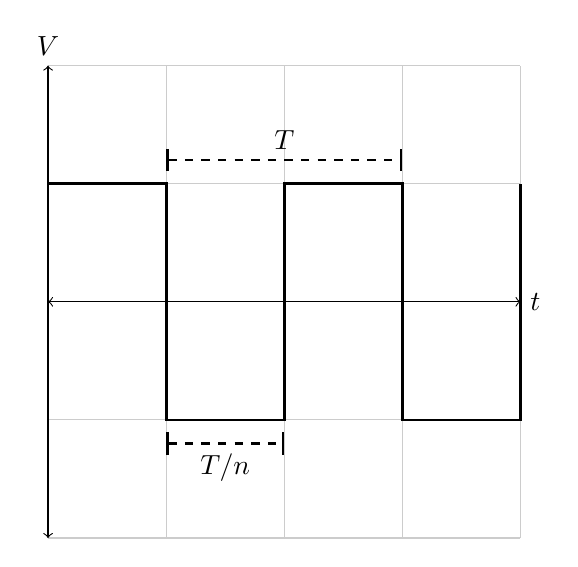
\begin{tikzpicture}[scale=1.5]

    \draw[thin,gray!40] (0,0) grid (4,4);
    
    
    \draw[<->] (0,2)--(4,2) node[right] {$t$};
    \draw[<->] (0,0)--(0,4) node[above]{$V$};

    \draw[line width=1pt,black](0,3)--(1,3)--(1,1)--(2,1)--(2,3)--(3,3)--(3,1)--(4,1)--(4,3);
    \draw[line width=1pt,black,|-|,dashed](1,3.2)--(3,3.2) node[midway,above]{$T$};
    \draw[line width=1pt,black,|-|,dashed](1,0.8)--(2,0.8) node[midway,below]{$T/n$};
\end{tikzpicture}

    \end{minipage}
    \begin{minipage}{0.49\textwidth}
        \centering
        \input{Plots/TriFC}
    \end{minipage}
   
    \caption{Señales de referencia}
    \label{fig:Señref}
\end{figure}

Como se puede observar en la figura\ref{fig:Señref} se asume que la señal cuadrada teniendo en cuenta que el ciclo negativo de la señal es de T/n\%.
Para la señal cuadrada la integral estará dada por:
\begin{equation}
    \begin{aligned}
         V_{rms}=&\sqrt{\frac{2}{T}\int_{0}^{\frac{T}{n}}V_{p}^2dt}\\
         V_{rms}=&\sqrt{\frac{2V_{p}^2\cdot\frac{\cancel{T}}{n}}{\cancel{T}}}\\
         V_{rms}=&\frac{V_{p}\sqrt{2}}{\sqrt{n}}
    \end{aligned}
\end{equation}
Teniendo en cuenta que la señal cuadrada medida en el experimento 3 su ciclo negativo es del 50\%:
\begin{equation}
    V_{rms}=V_{p}
\end{equation}
El factor $C_{eficaz}$ para una señal de este tipo es entonces 1.


Para señales triangulares:
\begin{equation}
    \begin{aligned}
         V_{rms}=&\sqrt{\frac{2}{T}(\int_{0}^{\frac{T}{4}}f_{(t)}^2dt+\int_{\frac{T}{4}}^{\frac{T}{2}}f_{(t)}^2dt)}\\
         V_{rms}=&\sqrt{\frac{2}{T}(\int_{0}^{\frac{T}{4}}(\frac{V_{p}}{T/4}\cdot t)^2)dt+\int_{\frac{T}{4}}^{\frac{T}{2}}((\frac{-V_{p}}{T/4}\cdot t)^2dt)}\\
          V_{rms}=&\sqrt{\frac{64V_{p}^2}{T^3}\int_{0}^{\frac{T}{4}}t^2dt}\\
          V_{rms}=&V_{p}\cdot\sqrt{\frac{64}{3T^3}\cdot(\frac{T}{4})^3}\\
          V_{rms}=&\frac{V_{p}}{\sqrt{3}}\\
    \end{aligned}
\end{equation}
El factor $C_{eficaz}$ para una señal de triangular es entonces $\frac{1}{\sqrt{3}}$.

Ahora el valor medio de estas señales rectificadas sera de:
\begin{equation}
    V_{media}=\frac{\int_{0}^{T} |f_{(t)}|dt}{T}
\end{equation}
\begin{figure}[H]
    \centering
    \begin{minipage}{0.49\textwidth}
        \centering
        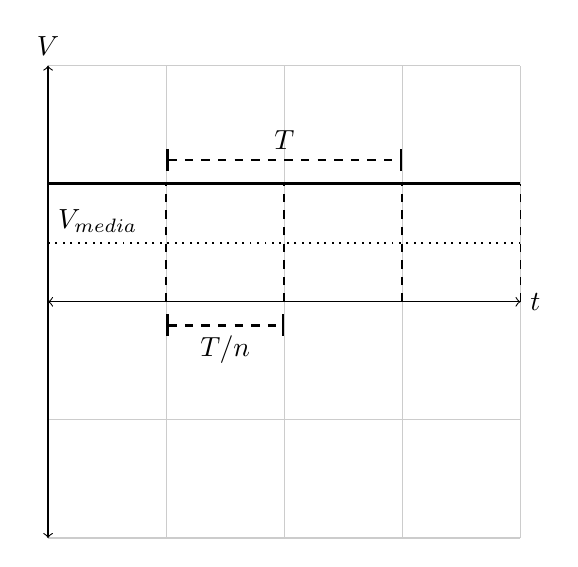
\begin{tikzpicture}[scale=1.5]

    \draw[thin,gray!40] (0,0) grid (4,4);
    
    
    \draw[<->] (0,2)--(4,2) node[right] {$t$};
    \draw[<->] (0,0)--(0,4) node[above]{$V$};
    \draw[line width=0.7pt,dotted](4,2.5)--(0,2.5) node[anchor=south west]{$V_{media}$};
    \draw[line width=1pt,black](0,3)--(4,3);
    \draw[line width=0.7pt,black,dashed](1,2)--(1,3);
    \draw[line width=0.7pt,black,dashed](2,2)--(2,3);
    \draw[line width=0.7pt,black,dashed](3,2)--(3,3);
    \draw[line width=0.7pt,black,dashed](4,2)--(4,3);
    \draw[line width=1pt,black,|-|,dashed](1,3.2)--(3,3.2) node[midway,above]{$T$};
    \draw[line width=1pt,black,|-|,dashed](1,1.8)--(2,1.8) node[midway,below]{$T/n$};
\end{tikzpicture}

    \end{minipage}
    \begin{minipage}{0.49\textwidth}
        \centering
        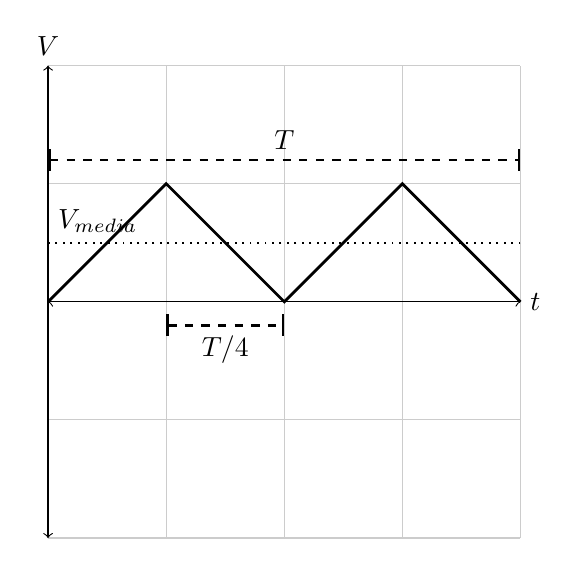
\begin{tikzpicture}[scale=1.5]

    \draw[thin,gray!40] (0,-2) grid (4,2);
    
    
    \draw[<->] (0,0)--(4,0) node[right] {$t$};
    \draw[<->] (0,-2)--(0,2) node[above]{$V$};
    \draw[line width=0.7pt,black,dotted](4,0.5)--(0,0.5) node[anchor=south west]{$V_{media}$};
    \draw[line width=1pt,black](0,0)--(1,1)--(2,0)--(3,1)--(4,0);
    \draw[line width=1pt,black,|-|,dashed](0,1.2)--(4,1.2) node[midway,above]{$T$};
    \draw[line width=1pt,black,|-|,dashed](1,-0.2)--(2,-0.2) node[midway,below]{$T/4$};
    
\end{tikzpicture}

    \end{minipage}
   
    \caption{Señales de referencia}
    \label{fig:Señref}
\end{figure}
Para la señal cuadrada el valor medio es simplemente de:
\begin{equation}
    V_{media}=V_p
\end{equation}
Por lo tanto el factor $C_{media}$ para una señal cuadrada sera de $1$

Y para la señal triangular será de :
\begin{equation}
    \begin{aligned}
         V_{media}=&2\cdot\frac{\int_{0}^{\frac{T}{4}} |f_{(t)}|dt}{T}\\
         V_{media}=&2\cdot\frac{\int_{0}^{\frac{T}{4}} \frac{V_{p}}{T/4}\cdot t dt}{T}\\
         V_{media}=&\frac{8V_{p}}{T^2}t^2|_{0}^{\frac{T}{4}}\\
         V_{media}=&\frac{V_{p}}{2}
    \end{aligned}
\end{equation}
El factor $C_{media}$ será entonces para esta señal $0.5$.

%Ya teniendo todos nuestros factores podemos construir las ecuaciones que el multímetro de valor medio debería utilizar para estas señales:
%\begin{equation}
%    \begin{cases}
%        V_{RMSCuad}=Vp\\
%        V_{RMSTrian}=Vp\cdot0.5772
%    \end{cases}
%\end{equation}
Una vez calculados las constantes $C_{media}$ y $C_{eficaz}$ de la forma cuadrada y rectangular, se procede calcular el factor de corrección $\kappa$ para cada forma. Se utilizará el despeje de la expresión \ref{eq:factorKappa}, dándonos como resultado los siguientes factores de corrección:
\begin{equation}
    \begin{cases}
        \kappa_{Cuad}=\frac{2\sqrt{2}}{\pi} \approx 0.900\\
        \kappa_{Tria}=\frac{4\sqrt{2}}{\pi\sqrt{3}} \approx 1.040
    \end{cases}
\end{equation}

Finalmente, para obtener el valor True RMS, solo debemos multiplicar el valor del multímetro de valor medio ($V_{RMSmedio}$), por el coeficiente que corresponda según la forma de onda (ecuación \ref{eq:corrCalcTrueRms}).

\begin{equation}
    V_{TrueRMS(Cuad)} = \kappa_{Cuad} \cdot V_{RMS(Cuad)}
\end{equation}
\begin{equation}
    V_{TrueRMS(Tria)} = \kappa_{Tria} \cdot V_{RMS(Tria)}
\end{equation}



















\vspace{3cm}
\section{Bibliografía}
\begin{itemize}
   \item \url{https://slideplayer.es/slide/16695348/}
   \item \url{https://www.tel.uva.es/personales/lib/osciloscopio.html#:~:text=Con%20este%20mismo%20pulsador%2C%20cada,la%20parte%20ascendente%20o%20descendente.}
   \item \url{https://www.fceia.unr.edu.ar/eca1/files/teorias/osciloscopio.pdf}
    \item \url{https://www.manualslib.com/manual/1574416/Bk-Precision-2120c.html}
\end{itemize}


\end{document}